\documentclass[11pt,dvipdfm]{article}

\usepackage[utf8]{inputenc}
\usepackage{deauthor,times,graphicx,hyperref}
\usepackage{subfig}
\usepackage{paralist}
\usepackage{multirow}
\usepackage{macros}

%for highlight changes
\usepackage{soul}

\begin{document}

\title{Geo-Replication: Fast If Possible, Consistent If Necessary\thanks{Student author are followed by faculty author names, both in alphabetical order. Cheng Li and Valter Balegas are the lead authors of the work.}}

\author{Valter Balegas$^1$, Cheng Li$^2$, Mahsa Najafzadeh$^4$, Daniel Porto$^{3}$, 
Allen Clement$^{2,5}$, Sérgio Duarte$^1$, \\
Carla Ferreira$^1$, Johannes Gehrke$^6$, Jo\~{a}o Leit\~{a}o$^1$, Nuno Preguiça$^1$, Rodrigo Rodrigues$^3$, \\
Marc Shapiro$^4$, Viktor Vafeiadis$^2$\\
\small $^1$NOVA LINCS, DI, FCT, Universidade NOVA de Lisboa
$^2$Max Planck Institute for Software Systems (MPI-SWS)\\
\small $^3$INESC-ID / IST, University of Lisbon 
$^4$Inria \& Sorbonne Universités, UPMC Univ Paris 06, LIP6\\
\small $^5$Currently at Google
$^6$Microsoft and Cornell University}

\graphicspath{{./figures/redblue/redblueOrder/}{./figures/}}

\maketitle

\begin{abstract}
Geo-replicated storage systems are at the core of current Internet services.\ Unfortunately, 
there exists a fundamental tension between consistency and performance for offering scalable 
geo-replication. Weakening consistency semantics leads to less coordination and consequently
a good user experience, but it may introduce anomalies such as state divergence and invariant violation.\ In 
contrast, maintaining stronger consistency precludes anomalies but requires more coordination.\ This 
paper discusses two main contributions to address this tension.\ First, RedBlue Consistency 
enables blue operations to be fast (and weakly consistent) while the remaining red operations 
are strongly consistent (and slow).\ We identify sufficient conditions for determining when 
operations can be blue or must be red.\ Second, Explicit Consistency further increases the space 
of operations that can be fast by restricting the concurrent execution of only the operations 
that can break application-defined invariants.\ We further show how to allow operations to complete 
locally in the common case, by relying on a reservation system that moves coordination off the 
critical path of operation execution.

%Main parts of this paper are from two papers: ~\cite{Li2012RedBlue} and ~\cite{Balegas2015Indigo}.

%In this paper, we introduce two pieces of our prior work defining a set of principles for
%reducing the amount of required coordination for geo-replicated systems by taking into account
%two important properties, namely state convergence and invariant preservation~\cite{Li2012RedBlue} and ~\cite{Balegas2015Indigo}.
\end{abstract}

\section{Introduction}

% Geo-replication is key technique, used by providers of major Internet services who deploy several DCs worldwide, and also accessible to anyone who can instantiate VM images in the DCs of cloud providers.
A geo-replicated system maintains copies of the service state across geographically dispersed locations.
%A geo-replicated system is a replicated service that runs replica instances in geographically dispersed locations. 
Geo-replication is not only employed today by virtually all the providers of major Internet services, who typically manage several data centers spread across the globe, but is also accessible to anyone outsourcing their computational needs to cloud providers, since cloud services allow computations or VMs to be instantiated in different data centers.

% There are at least two important reasons for geo-replicating. First is disaster tolerance. Example of data center problems. But another crucial reason is performance, as studies point out.
There are two main reasons for deploying geo-replicated systems. The first reason is disaster tolerance, i.e., the ability to tolerate the unplanned outage of an entire data center, due to catastrophic events such as natural disasters~\cite{dc-outages}. The second reason is to reduce the latency between the users and the machines that provide the service. The importance of this aspect is demonstrated by several studies that point out an inverse correlation between response times and user satisfaction for important Internet services such as search~\cite{Schurman2009latency}.

% http://www.informationweek.com/cloud/7-data-center-disasters-youll-never-see-coming/d/d-id/1320702
% http://www.computerworlduk.com/galleries/infrastructure/ten-datacentre-disasters-that-brought-firms-offline-3593580/

% Problem is that latency is at odds with consistency, you can either coordinate replicas and get strongly consistent view or get immediate but inconsistent replies.
However, there is a fundamental tension between latency and consistency: intuitively, ensuring strong consistency requires coordination between replicas before returning a reply to the user, while, alternatively, a fast response can be given without replica coordination, but only ensuring weak consistency guarantees. This tension has led the providers of global-scale Internet services to choose, for some parts of their services, storage systems offering weak consistency guarantees such as eventual consistency~\cite{dynamo}, and, for other components, systems with strong consistency such as serializability~\cite{Bernstein1987CCR}. 
%linearizability~\cite{spanner}.

% This paper summarizes in a unified way our two recent results in trying to achieve the best of both worlds: fast if possible and consistent when needed, ie minimal coordination to achieve desired semantics.
This paper revisits in a unified way two of our recent results in trying to achieve a balance between performance and consistency, by devising methods to build geo-replicated systems that introduce a small amount of coordination between replicas to achieve the desired semantics, i.e., systems that are fast when possible and consistent when necessary~\cite{Li2012RedBlue, Balegas2015Indigo}.
In the first result, we improve the performance of geo-replicated systems by (1) allowing different operations to execute in either a weakly consistent (fast) or strongly consistent (slow) manner; and (2) identifying a set of principles for making safe use
and increasing the space of fast operations.
In the second result, we further increase the space of operations that can execute fast by (1) identifying the operations that can break application invariants when executing concurrently; and (2) deploying concurrency control mechanisms that remove coordination from the critical path of operation execution, while preserving invariants.

% We start by expl system model; then simple scheme based on a two-level classification of ops, which already leads to some results; this is based on important notion of side effects commuting and we discuss how to achieve this using CRDTs; finally we present a more fine-grained classification that goes beyond just two consistency levels, and RW+conclude.
We start the presentation by laying out our terminology and system model in Section~\ref{sec:model}. We present an initial approach based on a coarse-grained classification into strong and weak consistency in Section~\ref{sec:redblue}. One key aspect of this approach is operation commutativity, and we explain how to achieve it using CRDTs in Section~\ref{sec:crdt}. Then we present an approach that makes use of fine-grained coordination between pairs of operations in Section~\ref{sec:indigo}. We discuss related work in section~\ref{sec:rel} and conclude in Section~\ref{sec:conc}.

\section{System model}
\label{sec:model}

%\hl{Note that the following paragraph is new. If you like it, then we have to change all terms ``site'' to ``replica'' throughout the whole paper.}

Our system model is that of a
fully replicated distributed system, where replicas are located in different data centers. Each replica follows a deterministic state machine: there is a set of operations $\mathcal{U}$, which manipulate
a set of reachable system states $\mathcal{S}$. %When operation $u$ is applied against a state $S$,
%it produces another state $S'$ (denoted $S'=S+u$). 
Each operation $u$ is initially submitted at a given replica (preferably in the closest data center), which we
call the \emph{origin replica} of $u$.
When the remaining replicas receive a request to replicate this operation, they will apply the operation against their local state. 

%% \hl{remove the whole paragraph. }Our system model is that of a
%% fully replicated distributed system, where replicas are located in $k$ sites denoted by $\textit{site}_0\ldots \textit{site}_{k-1}$. Each replica follows a deterministic state machine: there is a set of operations $\mathcal{U}$, which manipulate
%% a set of reachable system states $\mathcal{S}$. %When operation $u$ is applied against a state $S$,
%% %it produces another state $S'$ (denoted $S'=S+u$). 
%% Each operation $u$ is initially submitted at a given site, which we
%% call the \emph{primary site} of $u$ and denote $\textit{site}(u)$.
%% When a replica at the remaining sites receives a request to replicate this operation, that replica applies the operation against its local state. 


Throughout our explanation we will highlight two important properties
that the replicated system should obey. First, there is
the {\bf state convergence} property, which says that all the sites
that have executed the same set of operations against the same initial state are in the same final state.
%irrespectively of the order in which those operations were executed.
This is important to prevent a situation where
the system quiesces (no more updates are received) and
read-only queries return different results
depending on which sites the users are connected to.
%Another important property that consists of ensuring a good user
%experience is to preserve \textbf{causality}, both in terms of the monotonicity of user requests
%within a session and preserving causality across clients, which is key
%to enabling natural semantics~\cite{Petersen1997Flexible}. Additionally,
%operations invoked by client requests should return a {\bf single value}, precluding solutions that return a set of values
%corresponding to the outcome of multiple concurrent updates. 
The second property is to {\bf preserve application-specific invariants}, which comprise a specification for the behavior of the system.
%The second property is a specification for the behavior of the system, stating that the system should maintain a set of %application-specific
%{\bf invariants}. 
To define these, we introduce the primitive $\textit{valid}(S)$ to be {\it
  true} if state $S$ obeys these invariants and {\it false}
otherwise. 
%This allows us to introduce a basic notion of correctness
%of the implementation of a given service: an operation $u$ is {\it correct} if, for every valid state $S$, $S + u$ is also valid. 

\section{Mixing consistency levels in RedBlue consistency}
\label{sec:redblue}
%As mentioned before, to scale out the Internet services to meet their ever-growing user base, many
%recent storage systems have been proposed to replicate operations following a

In this section, we present a hybrid consistency model called RedBlue
consistency, where weakly consistent operations, labeled blue, can be executed at a
single replica and propagated in the background, with mostly no
coordination with concurrent actions at other replicas, while others, labeled red,
require a stronger consistency level and thus require cross-replica
coordination. RedBlue consistency is one of several systems that
propose labeling operations according to their consistency levels~\cite{Ladin1992LazyReplication, Singh2009Zeno,Li2012RedBlue,Pileus}, but improves on these systems by offering a precise method for labeling operations.

\begin{figure}[t!]
\centering
 \begin{minipage}[t]{0.45\columnwidth}
\centering
\subfloat[RedBlue order $O$ of operations]{
\centering
%\includegraphics[width=0.9\columnwidth]{figures/redblue/redblueOrder/redblueGlobalOrder.pdf}
\includegraphics[bb=0 0 206 140]{redblueGlobalOrder.pdf}
\label{fig:expositoryorder}
}
\end{minipage}
\hfill
 \begin{minipage}[t]{0.45\columnwidth}
\centering
\subfloat[Serializations of $O$]{
%\includegraphics[width=1.0\columnwidth]{figures/redblue/redblueOrder/redblueOrderSerial.pdf}
\includegraphics[bb=0 0 216 220]{redblueOrderSerial.pdf}
\label{fig:expositoryexecutionorder}
}
\end{minipage}
\caption{RedBlue order and serializations for a system spanning two
  sites. Operations marked with {\Large $\star$} are red, and
  operations marked with $\bigtriangleup$ are blue. Dotted arrows in \protect\subref{fig:expositoryorder} indicate the partial ordering of
operations. }
\label{fig:expositoryfigure}
\end{figure}

\subsection{Defining RedBlue consistency}

RedBlue consistency relies on three components: (1) a partitioning of operations into weakly consistent blue operations whose order of execution
can vary from site to site, and red operations that must
be executed in the same order at all sites, (2) a RedBlue order, which defines a partial order of
operations where red operations have to be ordered with respect to each other, and (3) a set of site-specific serializations (i.e., total orders)
in which the operations are locally applied. More precisely:

\begin{mydef}[RedBlue consistency]
A replicated system is {\em RedBlue consistent} if each site $i$ applies
operations according to a linear extension of a RedBlue order $O$ of the operations
that were invoked, where $O$ is a partial order among those operations with the requirement that red operations are totally ordered in $O$.
\label{def:rbct}
\end{mydef}

Figure~\ref{fig:expositoryfigure} shows a RedBlue order and two
serializations, i.e., the linear extensions of that order in which
operations are applied at two different sites. In systems where every operation is
labeled red, RedBlue consistency is equivalent to
serializability~\cite{Bernstein1987CCR}; in systems where every
operation is labeled blue, RedBlue consistency becomes a form of causal consistency~\cite{bayou,cops,
Mahajan2010Depot}, since the partial order conveys the necessary causality between operations.

When applying RedBlue consistency to an application, we would like to label all operations blue
to obtain best performance.
However, this could lead to state divergence and invariant violation, when operations are not commutative.
We describe a set of sufficient conditions to guide the classification of operations in order to safely use weak consistency
when possible.

%When applying RedBlue consistency
%to an application, the challenge is that we cannot arbitrarily label operations as blue (weakly consistent), since that might lead to
%breaking state convergence and invariant preservation. Therefore, to safely use blue operations, we must come up with a %set of sufficient conditions to guide the classification, which will
%be described next.

\subsection{Ensuring state convergence}
In the context of RedBlue consistency, we can formalize state convergence as follows:

\begin{mydef}[State convergence]
A RedBlue consistent system is state convergent if all serializations of
the underlying RedBlue order $O$ reach the same state $S$ w.r.t.\ any initial state $S_0$.
\end{mydef}

To find a correct labeling for maintaining state convergence while providing low latency access, we describe a
simple banking example, in which users may share an account that is modified
via three operations, namely {\tt deposit}, {\tt withdraw} and {\tt accrueinterest}\footnote{{\tt accrueinterest}
computes a new balance by multiplying the old balance value and (1 + {\tt interest rate}).}. Keeping in mind that one of the goals of RedBlue consistency is to make the target service as fast as possible, we tentatively
label all these operations blue. According to this labeling result, we construct a RedBlue order of deposits and interest accruals made by two users Alice and Bob and two possible serializations applied at both branches
of the bank, as shown in Figure~\ref{fig:bankexample}. This example shows that the labeling of these operations as described is not state convergent. This is because
RedBlue consistency allows the two sites to execute blue operations in a different order, but
two of the blue operations in the example are non-commutative, namely
{\tt deposit} and {\tt accrueinterest}. To prevent this situation, a sufficient condition to guarantee
state convergence in a system supporting RedBlue consistency is that every blue operation commutes with all other operations, blue or red.

\begin{figure}[t]
\centering
\begin{minipage}[t]{0.46\columnwidth}
\centering
\subfloat[\sf RedBlue order $O$ of operations issued by Alice and Bob ]{
%\includegraphics[width=0.9\columnwidth]{figures/redblue/redblueOrder/redblueOrderBank.pdf}
\includegraphics[bb=0 0 222 30]{redblueOrderBank.pdf}
\label{fig:simplebankrbo}
}
\end{minipage}
\hfill
\begin{minipage}[t]{0.46\columnwidth}
\centering
\subfloat[\sf Serializations of $O$ leading to diverged state]{
%\includegraphics[width=1.0\columnwidth]{figures/redblue/redblueOrder/redblueOrderBankSerial.pdf}
\includegraphics[bb=0 0 222 90]{redblueOrderBankSerial.pdf}
\label{fig:divergestate}
}
\end{minipage}
\caption{A RedBlue consistent account with initial balance of 100 and final diverged state}.
%\changebars{}{ (a) \RBo\ of
%  \operations\ issued by Alice and Bob. (b) Divergent causal serializations.}}
\label{fig:bankexample}
\end{figure}

However, when applying this condition to the banking example, it implies that we need to label all three operations red
({\tt deposit}, {\tt withdraw} and {\tt accrueinterest}).
This is equivalent to running the system under serializability, which requires coordination across replicas for executing all these operations.
To address the problem that it is difficult to find operations that commute with all other operations in the system, we observe that, in many cases,
while operations may not be commutative, we
can make the changes they induce on the system state to commute. In
the banking example, we can engineer {\tt accrueinterest} commute with the remaining two operations
by first computing the amount of interested accrued at the primary replica and then treating that value as a deposit.


To exploit this observation and increase operation commutativity, we propose a change to our
original system model,
where we split each original application operation $u$
into two components: a {\em generator operation} $g_u$ with no
side-effects, which is executed only at the primary site against some
system state $S$ and produces a {\em shadow operation} $h_u(S)$,
which is executed at every site (including the primary site). The
generator operation decides which state transitions should be made
while the shadow operation applies the transitions in a
state-indep\-endent manner.

\subsection{Preserving invariants}
%While the concept of shadow operation helps produce more commutative operations, it
%Concurrency introduces the problem of breaking application invariants. 
Although the concept of shadow operation helps produce more commutative operations, labeling too many
shadow operations as blue may introduce the problem of breaking application invariants. In the banking example, assuming that the shared bank account has an initial balance of $100$, if both Alice and Bob withdraw $70$ and $60$ respectively,
the final balance would be $-30$. This violates the
invariant that a bank balance should never be negative. To determine which shadow 
operations can be safely labeled blue, we begin by defining that a
shadow operation is invariant safe if, when applied to a valid state, it always transitions
the system into another valid state. This allows us to define the following
sufficient condition: a RedBlue consistent system preserves invariants (meaning that all its sites are always in valid states) if all shadow operations that are not invariant safe are labeled red (i.e., strongly consistent).

\if 0
\begin{theorem}[Invariant preservation]
A RedBlue consistent system preserves invariants (meaning that all its sites are always in valid states) if all operations that are not invariant safe are labeled red (i.e., strongly consistent).
\end{theorem}
\fi

\subsection{What can be blue?  What must be red?}
\label{ch:redblue:sect:labelmethod}
In summary, the two conditions above lead to the following procedure for deciding
which shadow operations can be
blue or must be red if a RedBlue consistent system is to provide both
state convergence and invariant preservation:
\begin{enumerate}%[leftmargin=0cm,itemindent=.5cm,labelwidth=\itemindent,labelsep=0cm,align=left]
\item For any pair of non-commutative shadow operations $h_u$ and $h_v$, label both $h_u$ and $h_v$ red.
\item For any shadow operation $h_u$ that is not invariant safe,
label $h_u$ red.
\item Label all remaining shadow operations blue.
\end{enumerate}


\section{State convergence}
\label{sec:crdt}
In the previous section we discussed how RedBlue consistency achieves state convergence by
relying on shadow operations that commute with each other.
With this approach, defining a new operation also implies
writing one or more commutative shadow operations, each of which corresponds to a distinct side effect.
The major challenge of doing this manual work
is that, in an application with a large number of operations, this process may be
complex and error-prone.

We now discuss an alternative principled approach to create commutative operations by design.
Our approach builds on conflict-free replicated data types (CRDTs)~\cite{crdts}, which are
specially-designed data structures that can be replicated and modified concurrently,
and include mechanisms to merge concurrent updates in a deterministic way.
Application operations consist of updates to these elementary data types, thus
guaranteeing state convergence.

\subsection{CRDTs}

A CRDT is a data type that can be replicated at multiple replicas. As such,
it defines an interface with a set of operations to read and to modify its state.
A CRDT replica can be modified by locally executing an update operation.
When different replicas of the same object are modified concurrently, they
temporarily diverge.
CRDTs have built-in support for achieving strong eventual consistency~\cite{crdts}, in which
all replicas will eventually reach the same (equivalent) state after applying
the same set of updates, without relying on a distributed conflict arbitration
process.

Two main flavors of CRDTs have been studied in the literature: operation-based CRDTs
and state-based CRDTs. For each of these, sufficient conditions for
achieving strong eventual consistency have been established.

In operation-based CRDTs (or commutative replicated data types), updates
are propagated by broadcasting operations to every replica in causal order.
Interestingly, this proposal matches the operation execution decomposition presented
in RedBlue consistency (Section~\ref{sec:redblue}), where operations are divided in two components, a {\em generator}
operation that executes in the local replica, has no side effect and produces a
{\em shadow} operation, which is propagated and executed in all replicas. 
The two types of operations are analogous to {\em prepare} and {\em downstream} operations
in the context of  operation-based CRDTs, respectively, with the main difference that shadow operations are assigned a consistency level in RedBlue consistency.
Similarly to the consequence of commutative shadow operations, the replicas of an operation-based CRDT converge to the same state after executing the same set of updates (in any order that respects causality)
if the execution of any two concurrent downstream operations commutes~\cite{crdts}.

A state-based CRDT (or convergent replicated data type) defines, in addition to
the operations to read and update its state, an operation to merge the
state of two replicas.
Replicas synchronize by exchanging the full replica states: when a new
state is received, the new updates are incorporated in the local replica
by executing the merge function.
It has been shown that the replicas of a state-based CRDT converge to the same state
after all replicas synchronize (directly or indirectly) if:
\begin{inparaenum}[(1)]
\item all the possible states of an object are partially ordered, forming a
join-semilattice;
\item the merge operation between two states is the semilattice join; and
\item an update monotonically increases the state according to the defined
partial order~\cite{crdts}.
\end{inparaenum}

\subsection{Examples}

CRDTs have been used in a number of research systems, such as Walter \cite{walter}
and SwiftCloud \cite{Zawirski15Write},
and commercial systems, such as Riak \cite{riak} and SoundCloud \cite{soundcloud}.
These systems include CRDTs that implement several data types, such as
registers, counters, sets, maps, and flags. For each such data type, it is possible to define and implement different semantics
to handle concurrent updates, leading to different CRDTs.
These semantics define which is the final state of a CRDT when
concurrent updates occur.
For example, for sets, it is possible to define an \emph{add-wins} semantics,
where, in the presence of a concurrent add and remove of some element $e$,
the final state will contain $e$ (or, more precisely, there exists an add of $e$
that does not happen before a remove of $e$).
It is also possible to define a \emph{remove-wins} semantics, where the remove will
win over a concurrent add.
Other semantics can also be implemented, such as a \emph{last-writer-wins} strategy where
an element will belong to the set or not depending on which was the last operation
executed, according to the order among operations.

When creating an application, an application developer must select the CRDT
with the most appropriate semantics for its goal.
For example, in the bank account example, the balance of an account can be modeled
as a counter and the set of accounts of a client can be maintained in an add-win set or map CRDT.

In general, an application operation will manipulate multiple data objects.
When using CRDTs, it is possible to maintain replicas of these objects in multiple nodes.
An operation can execute by accessing a single replica of each object it accesses.
These updates can later be propagated to other nodes, with CRDT rules guaranteeing
that the replicas of each object will converge to the same state.
By propagating the updates to all objects modified in an operation atomically,
it is possible to guarantee that all effects of an operation are observed at the
same time.

\paragraph{CRDTs for relational databases}

\begin{table}[t!]
\small
\centering
\begin{tabular}{|c|c|p{9.3cm}|}
\hline
SQL type & CRDT & Description \\
\hline
\hline
\multirow{2}{*}{FIELD*} & LWW &  Use last-writer-wins to solve concurrent updates\\\cline{2-3}
 & NUMDELTA  &  Add a delta to the numeric value \\\hline
\multirow{2}{*}{TABLE} & AOSET,                       UOSET,       & Sets with restricted operations (add, update, and/or remove). \\
& AUSET,              ARSET & Conflicting operations are logically executed by timestamp order.\\
\hline
\end{tabular}
\caption{Commutative replicated data types (CRDTs) for relational data. *
FIELD covers primitive types such as integer, float, double, datetime and string.}
\label{tab:crdts}
\end{table}

In relational databases, it is also possible to model data using CRDTs.
Table \ref{tab:crdts} presents the mapping proposed in SIEVE \cite{Li14Automating}.
Regarding table fields, we defined only two CRDTs. The \emph{LWW} CRDT can be
used with any field type and implements a \emph{last-writer-wins} strategy
for defining the final value of a field.
The \emph{NUMDELTA} CRDT can be used with numeric fields, and transforms each
update operation in a downstream operation that adds or subtracts
a constant to the value of the field.
This can be used to support account balances,
counters, etc.

A database table can be seen as a set of tuples.
In the general case, and following the semantics of the \emph{ARSET} CRDT, when concurrent
\emph{insert}, \emph{update} and \emph{delete} operations occur,
the following rules can be used:
\begin{inparaenum}[(1)]
\item concurrent inserts of tuples with the same key are treated as an insert followed
by a sequence of updates;
\item for concurrent updates, the rules defined for fields
are used to deterministically define the final value;
\item a delete will only take effect if no concurrent update or insert was executed.
\end{inparaenum}

While using CRDTs guarantees that all replicas converge to the same state, it does
not guarantee that the convergence rules executed independently by different CRDTs
maintain application invariants. Next, we show how we can address
this problem by restricting the concurrent execution of operations that can break
application invariants.
%, \hl{instead of serializing all non-invariant safe shadow operations.}



%The implementation of these CRDTs in a relational database is detailed
%elsewhere \cite{Li14Automating}.
%We note that although both CRDTs ensure convergence, their semantics
%differ significantly.
%For example, the first CRDT leads to a final state that does not
%reflect the effects of all update operations, while the second is only
%correct if all updates are commutative.
%
%For implementing these CRDTs in a relational database, we have added additional
%metadata to each table for recording for each field/row the timestamp of the
%last update and of the last delete operation.
%The information of a deleted row is not removed until it is known that no
%concurrent update was executed.
%
%We have to additionally modify the SQL operations to:
%\begin{inparaenum}[(1)]
%\item ignore deleted rows in select operations;
%\item update the metadata on insert, update and delete operations;
%\item use the metadata to implement to appropriate CRDT semantics.
%\end{inparaenum}




%Next, we will show how we can define CRDTs that are appropriate for handling
%concurrent updates in relational databases.

%While this approach guarantees that all replicas converge to the same state, it does
%not guarantee that the convergence rules executed independently by different CRDTs
%maintain application invariants. In Section~\ref{sec:indigo}, we show how we can address
%this problem by restricting the concurrent execution of operations that can break
%application invariants.
%
%\subsection{CRDTs for relational databases}
%
%We now show that data in a relational database can be modeled using
%CRDTs.
%Table \ref{tab:crdts} presents the mapping proposed in SIEVE \cite{Li14Automating}.
%
%\begin{table}[t!]
%\footnotesize
%\centering
%\begin{tabular}{|c|c|p{8cm}|}
%\hline
%SQL type & CRDT & Description \\
%\hline
%\multirow{3}{*}{FIELD*} & LWW &  Use last-writer-wins to solve concurrent updates\\\cline{2-3}
% & NUMDELTA  &  Add a delta to the numeric value \\\hline
%TABLE & AOSET,                       UOSET,                AUSET,              ARSET & Sets with restricted operations (add, update, and/or remove).
%Conflicting ops.\ are logically executed by timestamp order.\\
%\hline
%\end{tabular}
%\caption{Commutative replicated data types (CRDTs) for relational data. *
%FIELD covers primitive types such as integer, float, double, datetime and string.}
%\label{tab:crdts}
%\end{table}
%
%A database table can be seen as a set of tuples (with the key identifying
%the tuple).
%We have defined different semantics for these sets, that whether
%concurrent \emph{insert} and \emph{delete} SQL operations are allowed
%and how they are treated.
%For example, the \emph{AOSET} does not support \emph{delete} operations.
%The \emph{ARSET} supports concurrent \emph{insertion}, \emph{updates} and
%\emph{deletes}.
%Concurrent insertions of tuples with the same key are logically transformed
%in an insert followed by an update.
%For concurrent updates of the same data, the rules defined for fields
%are used to deterministically define the final value.
%A delete operation will only take effect if no concurrent update or insert
%is executed. Thus, the ARSET provides a semantics that can be characterized as
%update-wins, where any update to data wins over a concurrent delete.
%
%For table fields we have defined only two CRDTs. The \emph{LWW} CRDT can be
%used with any field type and implements a \emph{last-writer-wins} strategy where
%the update with the highest timestamp is selected for defining the final value of a field.
%
%For numeric fields, when a field is updated using a SQL update command,
%the programmer could have two different
%intentions in terms of what the update means and how concurrent
%updates should be handled:
%\begin{inparaenum}[(i)]
%\item the update can represent a delta to be
%added or subtracted from the current value (e.g., when updating the
%stock of a certain item), in which case all concurrent updates should
%be applied possibly in a different order at all replicas to ensure that no stock
%changes are lost, or
%\item it can be overwriting an old value with a new
%value (e.g., when updating the year of birth in a user profile), in
%which case an order for these updates should be arbitrated, and the last
%written value should prevail.
%\end{inparaenum}
%The latter case can be addressed using the \emph{LWW} CRDT, while
%for the former we have defined the \emph{NUMDELTA} CRDT, where each
%update operation is transformed in a downstream operation that adds or subtracts
%a constant to the value of the field.
%
%Both strategies ensure convergence, but their semantics differ significantly.
%For example, the second strategy leads to a final state that does not
%reflect the effects of all update operations, while the second is only
%correct if all updates are commutative.
%
%For implementing these CRDTs in a relational database, we have added additional
%metadata to each table for recording for each field/row the timestamp of the
%last update and of the last delete operation.
%The information of a deleted row is not removed until it is known that no
%concurrent update was executed.
%
%We have to additionally modify the SQL operations to:
%\begin{inparaenum}[(1)]
%\item ignore deleted rows in select operations;
%\item update the metadata on insert, update and delete operations;
%\item use the metadata to implement to appropriate CRDT semantics.
%\end{inparaenum}
%


\section{Preserving invariants with minimal coordination}
\label{sec:indigo}
%In section~\ref{sec:redblue}, we showed how to label shadow operations as
%blue or red, depending on whether they are commutative or might break invariants.
%While CRDTs can help programmers write commutative operations,
%this is still not sufficient to maintain many
%classes of application invariants.
%We also saw that executing operations in total order always ensures invariant
%preservation. Intuitively, this is because replicas execute operations one after another
%and can check that the pre-conditions of an operation are held globally.
As mentioned before, in the banking example, the {\tt withdraw} operation, despite
being commutative, cannot execute under weak consistency, as the concurrent
execution of multiple withdrawals can break the invariant that
the account balance cannot be negative. To avoid the possibility of breaking the invariant, RedBlue consistency would
label all withdrawals as red, requiring replicas to coordinate
the execution of every withdraw operation. In practice, however, only in a few cases the cumulative effects of all concurrent withdrawals
will surpass the actual balance of the account.

To relieve the strong constraint imposed by RedBlue consistency, we propose a more efficient
coordination plan: given some
account balance, replicas can coordinate beforehand to split the balance
among them. Until a replica consumes its allocated
share of the balance, it can execute operations locally, without
coordination with other replicas, with the guarantee that
the balance will not become negative, i.e., the application invariant will
not be broken.

The above idea has been previously explored in the
context of escrow transactions~\cite{BarbaraMilla1994Demarcation,ONeil1986Escrow}.
We revisit and generalize the concept of escrow transactions, to allow replicas to
assess the safety of operations without coordination when executing operations.
In our generalization, when replicas cannot ensure an operation is safe by
reading local state, they contact remote peers to update their vision of the
database to decide the fate of the operation.
In addition, we discuss how we avoid the coordination across sites for
all red operations, which is required for totally ordering them. Instead,
we identify a small set of coordination requirements between operations, and show
how to enforce those rules at runtime.

\subsection{Explicit Consistency in a nutshell}
We present a new consistency model, called Explicit Consistency, that extends
RedBlue consistency to avoid the coordination of red operations when possible.
The idea is that instead of labeling shadow operations as red or blue,
programmers specify the application invariants.
The system must execute operations while guaranteeing that these invariants are
not broken.

To this end, we propose the following methodology for creating applications
that adhere to Explicit Consistency.
First, programmers must specify the application invariants and operation effects.
Second, we provide a tool to analyze the specification of the application
and identify the pairs of conflicting shadow operations.
Non-conflicting shadow operations execute without any restrictions, as blue
operations. We include a library of CRDTs to help programmers define
commutative operations.
Third, for each pair of conflicting shadow operations,
the programmer can use a specialized concurrency control mechanism
that restricts the concurrent execution of these operations.
This mechanism executes coordination outside of the critical path of
operation execution, allowing these operations to execute locally
without the need to coordinate with other replicas.

The following sections provide additional details on these steps to
use the Explicit Consistency model.

%We present a new consistency model, called Explicit Consistency, that extends
%RedBlue consistency to avoid coordination of Red operations when possible.
%The idea is that programmers specify the application invariants, and,
%instead of labeling shadow operations as Red or Blue, the system determines which
%pairs of shadow operations conflict with each other and therefore require coordination.
%Non-conflicting shadow operations execute as Blue.
%For each pair of conflicting shadow operations, instead of labeling operations as Red,
%the programmer can use a specialized concurrency control mechanism that restricts the
%concurrent execution of these operations.
%%that avoids contacting remote replicas when possible.
%
%Our approach includes a tool to analyze the specification of the application. and a
%library of CRDTs that can be used to write
%execute a wide variety of shadow operations efficiently with safety.
%When safety can be ensured locally, shadow operations execute immediately without
%contacting any remote replica; otherwise, the runtime support of the
%application exchanges resources with remote peers to guarantee that the
%shadow operations can execute without violating any invariant.
%
%In the following sections we describe a methodology to build applications
%that use the Explicit Consistency model. The methodology comprises three steps:
%(1) the specification of the application; (2) the analysis of its conflicts; and (3) the
%instrumentation of the application to avoid them.

\subsection{Application specification}
Programmers specify application invariants and the post-conditions
of shadow operations as
first order logic expressions.
Invariants must be written as universally quantified formulas in prenex normal
form, while the grammar for specifying applications post-conditions is
restricted to predicate assignments, that assert the truth value of some
predicate, and function clauses, which define the relation between the value of
some predicate before and after the execution of the operation.
%The post-conditions of an operation cannot have alternative effects, i.e., they are always a conjunction of effects, but operations can fail without producing any effects.
% The specification of operations in this tool are similar to
%  shadow operations.
%The multiple effects of the same operation are expressed as a logical
%conjunction.

The code snippet in figure~\ref{fig:code-snippet} shows the specification of the
banking application.
We extended this example to illustrate different invariant violations.
In the extended version, clients must have a valid contract with the bank to
be able to access an account.
Clients might have multiple accounts and must close all of them before finishing the contract.
In Line 2, the invariant guarantees that an account balance is never negative.
In line 3, the invariant states that, for every open account, the account holder must be registered with the bank.
%In this example we used Java annotations to write the post-conditions of the operations.

\begin{figure}[t!]
\centering
 \begin{minipage}[b]{0.45\columnwidth}
\centering
\subfloat[Specification written with Java Annotations.]{
\centering
%\includegraphics[width=\textwidth]{figures/code-snippet-cropped.pdf}
\includegraphics[bb=0 0 220 180]{code-snippet-cropped.pdf}
\label{fig:code-snippet}
}
\end{minipage}
\hfill
\begin{minipage}[b]{0.53\columnwidth}
\centering
\subfloat[Conflicting pairs of operations for the Bank example.]{
%\includegraphics[width=\textwidth]{figures/conflict-table-cropped.pdf}
\includegraphics[bb=0 0 260 200]{conflict-table-cropped.pdf}
\label{fig:code-conflicts}
}
\end{minipage}
\caption{Bank application specification and analysis results.}
\end{figure}

\subsection{Analysis}
The analysis checks which are the shadow operations
whose concurrent execution might produce a
database state that is invalid with respect to the declared invariants.
Conceptually, for each pair of operations and for every valid state where
these operation can execute, the algorithm verifies if the execution of both
operations will lead to a state that is not valid according to the invariants
of the application.
%operations will lead to an invalid state where some application invariant
%does not hold.
%If this is the case, the concurrent execution of these operations can lead to
%an invariant violation.
Obviously, checking every pair of operations in every valid state
exhaustively is unfeasible. Instead, our algorithm relies in the
Z3 satisfiability modulo theory (SMT) solver to perform this verification
efficiently.
A full description of the algorithm is given in our prior publication~\cite{Balegas2015Indigo}.

%In an extension to our work, Gotsman et. al.~\cite{GotsmanConsistencyReason}
%prove that testing pairs of operations is sufficient for detecting if two
%operations might violate a defined invariant when executed concurrently.


%In order to do that, we use the Z3 satisfiability modulo theory (SMT) solver,
%to check, for every pair of shadow operations in the workload, $op_{i}, op_{j}$, if:
%\begin{itemize}
%    \item The execution of each operation produces a set of effects,
%        $E(op_{i})$ and $E(op_{j})$, that maintain the application invariants
%        when applied to the database individually.
%    \item There is a set of states $S$, in which both operations
%    		  $op_{i}, op_{j}$ can be applied together, i.e., that satisfy
%              the pre-conditions of both operations.
%    \item Both operation are invariant-safe, meaning that the effects of both operations
%        applied to all possible states $s_{i} \in S$ produces a new state
%        $s_{i} \cdot E(op_{i}) \cdot E(op_{j})$ that preserves the invariant.
%        Otherwise, the pair of operations is signaled as conflicting and the
%        reason is presented to the programmer.
%\end{itemize}

Figure~\ref{fig:code-conflicts} summarizes the conflicts in the example
of Figure~\ref{fig:code-snippet}:
two concurrent successful withdrawals might make the balance negative
(non-idempotence);
assigning and removing an account concurrently for the same user might leave
the system in an inconsistent state, because each shadow operation writes different
values for the predicate $userAccount(cId, aId)$ (opposing post-conditions);
and finally, the pair $createAccount(cId,$ $ aId)$ and $endContract(cId)$ might
violate the integrity constraint of line 3, because a new account is being
added to a user that is ending a contract with the bank.

%In the next section, we discuss how to address each of these conflicts
%efficiently.


%%The analysis algorithm checks which are the shadow operations
%%whose concurrent execution might produce a
%%database state that is invalid with respect to the declared invariants.
%%In order to do that, we use the Z3 satisfiability modulo theory (SMT) solver,
%%to check, for every pair of shadow operations in the workload, $op_{i}, op_{j}$, if:
%%\begin{itemize}
%%    \item The execution of each operation produces a set of effects,
%%        $E(op_{i})$ and $E(op_{j})$, that maintain the application invariants
%%        when applied to the database individually.
%%    \item There is a set of states $S$, in which both operations
%%    		  $op_{i}, op_{j}$ can be applied together, i.e., that satisfy
%%              the pre-conditions of both operations.
%%    \item Both operation are invariant-safe, meaning that the effects of both operations
%%        applied to all possible states $s_{i} \in S$ produces a new state
%%        $s_{i} \cdot E(op_{i}) \cdot E(op_{j})$ that preserves the invariant.
%%        Otherwise, the pair of operations is signaled as conflicting and the
%%        reason is presented to the programmer.
%%\end{itemize}
%%
%%A full description of the algorithm is given in our prior publication~\cite{Balegas2015Indigo}, and,
%%in a related piece of work~\cite{GotsmanConsistencyReason}, the authors prove that testing pairs of
%%operations is sufficient for detecting if two operations might violate a defined
%%invariant when executed concurrently.
%%
%%Figure~\ref{fig:code-conflicts} summarizes the conflicts in the example:
%%two concurrent successful withdraw shadow operations might make the balance negative
%%(non-idempotence);
%%assigning and removing an account concurrently for the same user might leave
%%the system in an inconsistent state, because each shadow operation writes different
%%values for the predicate $userAccount(cId, aId)$ (opposing post-conditions);
%%and finally, the pair $createAccount(cId,$ $ aId)$ and $endContract(cId)$ might
%%violate the integrity constraint of line 3, because a new account is being
%%added to a user that is ending its contract with the bank.
%%
%%%In the next section, we discuss how to address each of these conflicts
%%%efficiently.

\subsection{Code instrumentation}
After identifying which operations can lead to conflicts, the programmer
must instrument the application to avoid them.

Some conflicts can be handled by simply relying on CRDTs to automatically solve
them.
For example, our analysis can report that operations have 
opposing post-conditions: e.g., operations {\tt assignAccout} and {\tt remAccount}
assign the value \textit{true} and \textit{false} to predicate $userAccount(cId, aId)$.
In this situation, the programmer can choose a preferred value for the
predicate and use a CRDT that automatically implements the selected
decision\footnote{In our
experience, boolean predicates can be implemented using Set CRDTs with
add-wins and remove-wins policies to enforce that the corresponding 
predicate becomes true or false
respectively.}.

Other conflicts must be handled by restricting the concurrent execution of 
operations that can cause invariants to be broken. To this end, we provide a set 
of specialized reservation-based concurrency control mechanisms.

For conflicts on numeric invariants, like the one that withdraw causes,
% with the invariant that specifies that the balance should be non-negative, 
we support an escrow reservation for allowing some decrements of numeric 
values to execute without coordination.
In an escrow reservation, each replica is assigned a budget of decrements,
based on the initial value of the data.
In our example, when a replica receives a withdraw request, if the local 
budget is sufficient, the generator operation executes immediately 
without coordination, generating a shadow operation that decrements 
the balance.
This local execution is safe, guaranteeing that the invariant still holds
after executing all concurrent operations, because the sum 
of the budgets of all replicas is equal to the value of the initial value.
If the local budget is not enough to satisfy the request, the replica needs to
contact remote replicas to increase its budget, until it can satisfy the request.
If that is not possible, because there are not enough resources globally,
then the generator operation fails, generating no shadow operation.

For conflicts on generic invariants, we include a multi-value lock 
reservation. This lock can be in one of the following three states: 
(1) shared forbid, giving the shared right to forbid some action to occur; 
(2) shared allow, giving the shared right to allow some action to occur; 
(3) exclusive allow, giving the exclusive right to execute some action.
The idea is that, for a conflicting pair of operations, $(o_1,o_2)$, 
the lock will be associated with the execution of one of the operations, 
say $o_1$.
To execute $o_1$, a replica must hold the lock in the shared allow mode.
This right can be shared by multiple replicas.
To execute $o_2$, a replica must hold the lock in the shared forbid mode.
As before, when executing the generator operation, if the replica already
holds the necessary locks (in the required mode to execute the operation), 
it can execute locally and generate the corresponding shadow operation.
If not, it must contact other replicas to obtain the necessary locks.

Besides these two locks, we also proposed other locks that can
efficiently restrict the concurrent execution of operations that conflict 
in other types of invariants, including conditions on the number of elements
that satisfy a given condition and disjunctions.
In a related work, Gotsman et. al.~\cite{GotsmanConsistencyReason}
have shown how to prove that a given set of locks is sufficient
for maintaining invariants.




%%For numerical conflicts, like the one in the $withdraw(cId, aId, amount)$, we
%%provide the bounded counter CRDT~\cite{Balegas2015Counter}, which assigns to 
%%each replica a budget of decrement operations that each replica can execute.
%%When a replica receives a withdraw request, if the local budget is sufficient
%%to satisfy it, the generator operation executes immediately without coordination.
%%The local execution of the generator operation is safe because the sum of the budgets of
%%each replica is equal to the value of the counter.
%%If the local budget is not enough to satisfy the request, the replica needs to
%%contact remote peers to increase its budget, until it allows to satisfy the request.
%%If that is not possible, because there are not enough resources globally,
%%then the generator operation can fall back to safely going through the failed path,
%%which generates an invariant safe shadow operation---no-op.%no effects that might break invariants.
%%
%%For the second conflict reported by the analysis, the shadow operations have
%%opposing post-conditions: the value \textit{true} and \textit{false} are
%%assigned to the predicate $userAccount(cId, aId)$.
%%In this situation, the programmer must choose a preferred value for that
%%predicate.
%%In order to do so, the programmer must switch the data type implementing this
%%predicate to a CRDT and use the desired convergence policy~\footnote{In our
%%experience, boolean predicates can be implemented using Set CRDTs and
%%add-wins/remove-wins policies to enforce that the corresponding predicate becomes true/false
%%respectively.}
%%
%%When there is no conflict resolution mechanism for a specific type of invariant violations,
%%the programmer can control the execution of conflicting operations with CRDT tokens.
%%The idea of these tokens is that, for a conflicting pair of shadow operations, the replica
%%must hold a token to execute one of the corresponding generator operations.
%%The token only allows one of the corresponding generator operations to execute at a time,
%%the other is forbidden.
%%The token can act as a mutex, or multiple replicas can hold a piece of it to
%%execute the allowed generator operation concurrently with other peers.
%%When some replica needs to execute the generator operation that is being forbidden by the
%%token, it must coordinate with remote peers to revoke any permissions to
%%execute the current generator operation, and with this revocation they
%%incorporate all the shadow operations from the remote sites that still had
%%not been locally executed.
%%The runtime system must use some policy to ensure that all replicas eventually
%%satisfy their requests.




%\subsection{Comparison to RedBlue consistency}



\section{Related work}
\label{sec:rel}

Many cloud storage systems supporting geo-replication have emerged in recent years.
Some of these systems offer variants of eventual consistency, where operations produce
responses right after being executed in a single data center (usually the closest
one) and are replicated in the background, so that user observed latency is improved~\cite{dynamo,cops,eiger,chainreaction,cassandra}.
%This approach is very popular, as it allows low latency for end-users, by having data centers in multiple locations scattered across the globe and executing %users' operation in the closest datacenter.
These variants target different requirements, such as: reading a causally consistent view of the database (causal consistency) \cite{cops,chainreaction,orbe,bolton}; supporting limited transactions where a set of updates are made visible atomically \cite{eiger,ramp}; supporting application-specific or type-specific reconciliation with no lost updates \cite{dynamo,cops,walter,riak}, etc.

While some systems implement eventual consistency by relying on a simple last-writer-wins
strategy, others have explored the semantics of applications (and data types).
Semantic types \cite{semanticDDB} have been used for building non-serializable 
schedules that preserve consistency in distributed databases. 
Conflict-free replicated data types~\cite{crdts} explore commutativity 
for enabling the automatic merge of concurrent updates to the same data types.

Eventual consistency is insufficient for some applications that require 
some operations to execute under strong consistency for correctness. 
To this end, several systems support strong consistency. 
Spanner provides strong consistency for the whole database, at the cost
of incurring coordination overhead for all updates  \cite{spanner}. 
Transaction chains support transaction serializability with latency
proportional to the latency to the first replica that the corresponding transaction accesses~\cite{transactionchains}.
MDCC \cite{mdcc} and Replicated Commit \cite{replicatedcommit} propose optimized approaches for executing transactions but still incur inter-data center latency for committing transactions.

%Systems that provide strong consistency incur in coordination overhead that increases latency of operations. 
Some systems combine the benefits of weak and strong consistency models by allowing both levels to coexist. 
In Walter \cite{walter}, transactions that can execute under weak consistency run fast, without needing to coordinate with other datacenters.
Bayou \cite{bayou} and Pileus \cite{Pileus} allow operations to read data with different consistency levels, from strong to eventual consistency.
PNUTS \cite{pnuts} and DynamoDB \cite{dynamoDB} also combine weak consistency with per-object strong consistency relying on conditional writes, where a write fails in the presence of concurrent writes.
RedBlue consistency also combines weak and strong consistency in the same system. 
Unlike other systems, RedBlue consistency splits operations into
generator and shadow parts to allow more 
operations to commute, and define a procedure to help programmers labeling shadow operations 
as weak or strong.

Escrow transactions \cite{ONeil1986Escrow} offer a mechanism for
enforcing numeric invariants under concurrent execution of transactions.
By enforcing local invariants in each transaction, they can guarantee that a
global invariant is not broken.
This  idea can be applied to other data types, and it has been 
explored for supporting disconnected operation
in mobile computing \cite{Walborn95Semantics,mobisnap,exo-leasing}.
Balegas et al.~\cite{Balegas2015Counter} proposed the bounded counter CRDT
that can be used to enforce numeric invariants in weakly consistent cloud
databases.
The demarcation protocol \cite{BarbaraMilla1994Demarcation} aims at maintaining invariants
in distributed databases. 
Although its underlying protocols are similar to escrow-based 
approaches, it focuses on maintaining invariants across different objects.
Warranties \cite{warranties} provide time-limited assertions over the database state, which can improve latency of read operations in cloud storages.
Indigo builds on similar ideas for enforcing application invariants, 
but it is the first piece of work
to provide an approach that, starting from application invariants expressed in first-order
logic, leads to the deployment of the appropriate techniques for enforcing such 
invariants in a geo-replicated weakly consistent data store. 
Gotsman et. al. \cite{GotsmanConsistencyReason} propose a proof rule 
for establishing that the use of a given set of techniques is
sufficient to ensure the preservation of invariants.

The static analysis of code is a standard technique used extensively for 
various purposes, 
including in a context similar to ours.
SIEVE \cite{Li14Automating} combines static and dynamic analysis to infer
which operations should use strong consistency and which operations should
use weak consistency in a RedBlue system \cite{Li2012RedBlue}.
Roy et al. \cite{Roy14Writes} present an analysis algorithm that
describes the semantics of transactions.
These works are complementary to ours, since the proposed techniques
could be used to automatically infer application side effects.
%The latter work also proposes an algorithm to allow replicas to
%execute transactions independently by defining conditions that must
%be met in each replica. 
%Whenever an operation cannot commit locally, 
%a new set of conditions is computed and installed in all replicas
%using two-phase commit. 
%In \oursystem{}, replicas can exchange rights in a peer-to-peer manner. 



\section{Conclusion}
\label{sec:conc}

In this paper we summarized two of our recent results in addressing the fundamental tension
between latency and consistency in geo-replicated systems. First,
RedBlue consistency~\cite{Li2012RedBlue} offers fast geo-replication by
presenting sufficient conditions that allow programmers to safely separate
weakly consistent (fast) operations from strongly consistent (slow) ones in
a coarse-grained manner. To increase the space of potential fast operations
and simplify the programmer's task of defining commutative operations, 
we propose the use of conflict-free replicated data types. Second,  Explicit Consistency~\cite{Balegas2015Indigo}
enables programmers to make fine-grained decisions on consistency level assignments
by connecting application invariants to ordering conflicts between pairs of operations,
and explores efficient reservation techniques for coordinating conflicting operations with
low cost.

%Our first work, RedBlue consistency~\cite{Li2012RedBlue}, enables blue
%operations to be fast (and eventually consistent) while
%the remaining red operations are strongly consistent
%(and slow). 
%We have discussed the conditions when operations
%can be blue and must be red.
%To increases the space of potential blue operations
%and simplify the programmer's task of defining commutative operations, 
%we propose the use of conflict-free replicated data types.
%Our second work, Explicit Consistency~\cite{Balegas2015Indigo}, 
%further increases the space of operations that can be fast by 
%only restricting the concurrent execution of the operations that can break
%application-defined invariants.
%We propose a methodology to, from the application-defined invariants, 
%deploy a reservation system that allow operations to complete locally in the
%common case, by moving coordination off the critical path of operation execution.

%Main parts of this paper are from two papers: ~\cite{Li2012RedBlue} and ~\cite{Balegas2015Indigo}.


%NOTE: the description of redblue and explicit in abstract and conclusion looks very similar. 
%bibliography needs to be fixed.... I have just copied the bib file from indigo paper to the end of our bib file... some references may be duplicated.

\section*{Acknowledgments}

The research of Rodrigo\ Rodrigues is supported by the European Research Council under an ERC Starting Grant.
This research was also supported in part 
    by EU FP7 SyncFree project (609551),
%    \href{http://syncfree.lip6.fr/}{609\,551 SyncFree} (2013--2016), %
    %\usebox{\EUflagBW}, 
    FCT/MCT SFRH/BD/87540/2012, PEst-OE/ EEI/ UI0527/ 2014, 
NOVA LINCS (UID/CEC/04516/2013), and INESC-ID (UID/CEC/50021/2013).


\begin{thebibliography}{10} 
\itemsep=1pt 
\begin{small}


\bibitem{dc-outages}
{7 Data Center Disasters You'll Never See Coming}.
\newblock
  \url{http://www.informationweek.com/cloud/7-data-center-disasters-youll-never-see-coming/d/d-id/1320702}.
\newblock Accessed Feb-2016.

\bibitem{riak}
Using data types -- riak documentation.
\newblock \url{http://docs.basho.com/riak/latest/dev/using/data-types/}.
\newblock Accessed Feb-2016.

\bibitem{soundcloud}
Consistency without Consensus: CRDTs in Production at SoundCloud.
\newblock  \url{http://www.slideshare.net/InfoQ/consistency-without-consensus-crdts-in-production-at-soundcloud}
\newblock Accessed Feb-2016.

\bibitem{chainreaction}
S.~Almeida, J.~Leit\~{a}o, and L.~Rodrigues.
\newblock {Chain{R}eaction: A Causal+ Consistent Datastore Based on Chain
  Replication}.
  \newblock In {\em EuroSys '13}, 85--98, 2013. ACM.
%\newblock In {\em Proc.\ 8th ACM European Conf.\ on Computer Systems}, EuroSys
%  '13, pages 85--98, New York, NY, USA, 2013. ACM.

\bibitem{ramp}
P.~Bailis, A.~Fekete, J.~M. Hellerstein, A.~Ghodsi, and I.~Stoica.
\newblock {Scalable Atomic Visibility with RAMP Transactions}.
\newblock In {\em SIGMOD '14}, 27--38, 2014. ACM.
%\newblock In {\em Proc.\ 2014 ACM SIGMOD Int.\ Conf.\ on Management of Data},
%  SIGMOD '14, pages 27--38, New York, NY, USA, 2014. ACM.

\bibitem{bolton}
P.~Bailis, A.~Ghodsi, J.~M. Hellerstein, and I.~Stoica.
\newblock {Bolt-on Causal Consistency}.
\newblock In {\em SIGMOD '13}, 761--772, 2013. ACM.
%  \newblock In {\em Proc.\ 2013 ACM SIGMOD Int.\ Conf.\ on Management of Data},
%  SIGMOD '13, pages 761--772, New York, NY, USA, 2013. ACM.

\bibitem{Balegas2015Indigo}
V.~Balegas, S.~Duarte, C.~Ferreira, R.~Rodrigues, N.~Pregui\c{c}a,
  M.~Najafzadeh, and M.~Shapiro.
\newblock Putting consistency back into eventual consistency.
\newblock In {\em EuroSys '15}, 6:1--6:16, 2015. ACM.
%  \newblock In {\em Proceedings of the Tenth European Conference on Computer
%  Systems}, EuroSys '15, pages 6:1--6:16, New York, NY, USA, 2015. ACM.

\bibitem{Balegas2015Counter}
V.~Balegas, D.~Serra, S.~Duarte, C.~Ferreira, M.~Shapiro, R.~Rodrigues, and
  N.~Preguica.
\newblock Extending eventually consistent cloud databases for enforcing numeric
  invariants.
\newblock In {\em SRDS '15}, 31--36, Sept 2015.
%  \newblock In {\em Reliable Distributed Systems (SRDS), 2015 IEEE 34th Symposium
%  on}, pages 31--36, Sept 2015.

\bibitem{BarbaraMilla1994Demarcation}
D.~Barbar\'{a}-Mill\'{a} and H.~Garcia-Molina.
\newblock The demarcation protocol: A technique for maintaining constraints in
  distributed database systems.
\newblock {\em The VLDB Journal}, 3(3):325--353, July 1994.

\bibitem{Bernstein1987CCR}
P.~A. Bernstein, V.~Hadzilacos, and N.~Goodman.
\newblock {\em Concurrency Control and Recovery in Database Systems}.
\newblock Addison-Wesley, 1987.

\bibitem{pnuts}
B.~F. Cooper, R.~Ramakrishnan, U.~Srivastava, A.~Silberstein, P.~Bohannon,
  H.-A. Jacobsen, N.~Puz, D.~Weaver, and R.~Yerneni.
\newblock {PNUTS: Yahoo!'s Hosted Data Serving Platform}.
\newblock {\em Proc. VLDB Endow.}, 1(2):1277--1288, Aug. 2008.

\bibitem{spanner}
J.~C. Corbett, J.~Dean, M.~Epstein, A.~Fikes, C.~Frost, J.~J. Furman,
  S.~Ghemawat, A.~Gubarev, C.~Heiser, P.~Hochschild, W.~Hsieh, S.~Kanthak,
  E.~Kogan, H.~Li, A.~Lloyd, S.~Melnik, D.~Mwaura, D.~Nagle, S.~Quinlan,
  R.~Rao, L.~Rolig, Y.~Saito, M.~Szymaniak, C.~Taylor, R.~Wang, and
  D.~Woodford.
\newblock {Spanner: Google's Globally-distributed Database}.
\newblock In {\em OSDI '12}, 251--264, 2012. USENIX
  Association.
%\newblock In {\em Proc.\ 10th USENIX Conf.\ on Operating Systems Design and
%  Implementation}, OSDI'12, pages 251--264, Berkeley, CA, USA, 2012. USENIX
%  Association.

\bibitem{dynamo}
G.~DeCandia, D.~Hastorun, M.~Jampani, G.~Kakulapati, A.~Lakshman, A.~Pilchin,
  S.~Sivasubramanian, P.~Vosshall, and W.~Vogels.
\newblock {Dynamo: Amazon's Highly Available Key-value Store}.
\newblock In {\em  SOSP '07}, 205--220, 2007. ACM.
%\newblock In {\em Proc.\ 21st ACM SIGOPS Symp.\ on Operating Systems
% Principles}, SOSP '07, pages 205--220, New York, NY, USA, 2007. ACM.

\bibitem{orbe}
J.~Du, S.~Elnikety, A.~Roy, and W.~Zwaenepoel.
\newblock {Orbe: Scalable Causal Consistency Using Dependency Matrices and
  Physical Clocks}.
\newblock In {\em  SOCC '13}, 11:1--11:14, 2013. ACM.
%  \newblock In {\em Proc.\ 4th Annual Symp.\ on Cloud Computing}, SOCC '13, pages
%  11:1--11:14, New York, NY, USA, 2013. ACM.

\bibitem{semanticDDB}
H.~Garcia-Molina.
\newblock Using semantic knowledge for transaction processing in a distributed
  database.
\newblock {\em ACM Trans. Database Syst.}, 8(2):186--213, June 1983.

\bibitem{GotsmanConsistencyReason}
A.~Gotsman, H.~Yang, C.~Ferreira, M.~Najafzadeh, and M.~Shapiro.
\newblock 'cause i'm strong enough: Reasoning about consistency choices in
  distributed systems.
\newblock In {\em POPL 2016}, 371--384, 2016. ACM.
%  \newblock In {\em Proceedings of the 43rd Annual ACM SIGPLAN-SIGACT Symposium
%  on Principles of Programming Languages}, POPL 2016, pages 371--384, New York,
%  NY, USA, 2016. ACM.

\bibitem{mdcc}
T.~Kraska, G.~Pang, M.~J. Franklin, S.~Madden, and A.~Fekete.
\newblock {MDCC: Multi-data Center Consistency}.
\newblock In {\em EuroSys '13}, 113--126, 2013. ACM.
%  \newblock In {\em Proc.\ 8th ACM European Conf.\ on Computer Systems}, EuroSys
%  '13, pages 113--126, New York, NY, USA, 2013. ACM.

\bibitem{Ladin1992LazyReplication}
R.~Ladin, B.~Liskov, L.~Shrira, and S.~Ghemawat.
\newblock Providing high availability using lazy replication.
\newblock {\em ACM Trans. Comput. Syst.}, 10(4):360--391, Nov. 1992.

\bibitem{cassandra}
A.~Lakshman and P.~Malik.
\newblock {Cassandra: A Decentralized Structured Storage System}.
\newblock In {\em SIGOPS Oper. Syst. Rev.}, 44(2):35--40, 2010.

\bibitem{Li14Automating}
C.~Li, J.~Leit{\~a}o, A.~Clement, N.~Pregui{\c c}a, R.~Rodrigues, and
  V.~Vafeiadis.
\newblock Automating the choice of consistency levels in replicated systems.
\newblock In {\em ATC '14},
  281--292, 2014. USENIX Association.
%  \newblock In {\em 2014 USENIX Annual Technical Conference (USENIX ATC 14)},
%  pages 281--292, Philadelphia, PA, June 2014. USENIX Association.

\bibitem{Li2012RedBlue}
C.~Li, D.~Porto, A.~Clement, J.~Gehrke, N.~Pregui\c{c}a, and R.~Rodrigues.
\newblock {Making Geo-replicated Systems Fast As Possible, Consistent when
  Necessary}.
\newblock In {\em OSDI '12}, 265--278, 2012. USENIX
  Association.
%\newblock In {\em Proc.\ 10th USENIX Conf.\ on Operating Systems Design and
%  Implementation}, OSDI'12, pages 265--278, Berkeley, CA, USA, 2012. USENIX
%  Association.  
  

\bibitem{warranties}
J.~Liu, T.~Magrino, O.~Arden, M.~D. George, and A.~C. Myers.
\newblock Warranties for faster strong consistency.
\newblock In { \em NSDI '14}, 2014. USENIX Association.
%\newblock In {\em Proc.\ 11th USENIX Conf.\ on Networked Systems Design and
%  Implementation}, {NSDI'14}, Berkeley, CA, USA, 2014. USENIX Association.

\bibitem{cops}
W.~Lloyd, M.~J. Freedman, M.~Kaminsky, and D.~G. Andersen.
\newblock {Don't Settle for Eventual: Scalable Causal Consistency for Wide-area
  Storage with COPS}.
\newblock In { \em SOSP  '11}
, 401--416, 2011. ACM.
%\newblock In {\em Proc.\ 23d ACM Symp.\ on Operating Systems Principles}, SOSP
%  '11, pages 401--416, New York, NY, USA, 2011. ACM.

\bibitem{eiger}
W.~Lloyd, M.~J. Freedman, M.~Kaminsky, and D.~G. Andersen.
\newblock {Stronger Semantics for Low-latency Geo-replicated Storage}.
\newblock In {\em  NSDI '13}, 313--328, 2013. USENIX
  Association.
%  \newblock In {\em Proc.\ 10th USENIX Conf.\ on Networked Systems Design and
%  Implementation}, {NSDI'13}, pages 313--328, Berkeley, CA, USA, 2013. USENIX
%  Association.

\bibitem{Mahajan2010Depot}
P.~Mahajan, S.~Setty, S.~Lee, A.~Clement, L.~Alvisi, M.~Dahlin, and M.~Walfish.
\newblock Depot: cloud storage with minimal trust.
\newblock In {\em OSDI}, 2010.

\bibitem{replicatedcommit}
H.~Mahmoud, F.~Nawab, A.~Pucher, D.~Agrawal, and A.~El~Abbadi.
\newblock {Low-latency Multi-datacenter Databases Using Replicated Commit}.
\newblock {\em Proc. VLDB Endow.}, 6(9):661--672, 2013.

\bibitem{ONeil1986Escrow}
P.~E. O'Neil.
\newblock The escrow transactional method.
\newblock {\em ACM Trans. Database Syst.}, 11(4):405--430, Dec. 1986.

\bibitem{mobisnap}
N.~Pregui\c{c}a, J.~L. Martins, M.~Cunha, and H.~Domingos.
\newblock {Reservations for Conflict Avoidance in a Mobile Database System}.
\newblock In {\em MobiSys '03}, 43--56, 2003. ACM.
%  \newblock In {\em Proc.\ 1st Int.\ Conf.\ on Mobile Systems, Applications and
%  Services}, MobiSys '03, pages 43--56, New York, NY, USA, 2003. ACM.

\bibitem{Roy14Writes}
S.~Roy, L.~Kot, G.~Bender, B.~Ding, H.~Hojjat, C.~Koch, N.~Foster, and
  J.~Gehrke.
\newblock The homeostasis protocol: Avoiding transaction coordination through
  program analysis.
\newblock In {\em SIGMOD '15}, 1311--1326, 2015.
%\newblock In {\em Proceedings of the 2015 {ACM} {SIGMOD} International
%  Conference on Management of Data, Melbourne, Victoria, Australia, May 31 -
%  June 4, 2015}, pages 1311--1326, 2015.  

\bibitem{Schurman2009latency}
E.~Schurman and J.~Brutlag.
\newblock Performance related changes and their user impact. {P}resented at
  velocity web performance and operations conference.
\newblock \url{http://slideplayer.com/slide/1402419/}, 2009.

\bibitem{crdts}
M.~Shapiro, N.~Pregui\c{c}a, C.~Baquero, and M.~Zawirski.
\newblock {Conflict-free Replicated Data Types}.
\newblock In {\em SSS '11}, 386--400, 2011. Springer-Verlag.
%\newblock In {\em Proc.\ 13th Int.\ Conf.\ on Stabilization, Safety, and
%  Security of Distributed Systems}, SSS'11, pages 386--400, Berlin, Heidelberg,
%  2011. Springer-Verlag.  
  

\bibitem{exo-leasing}
L.~Shrira, H.~Tian, and D.~Terry.
\newblock {Exo-leasing: Escrow Synchronization for Mobile Clients of Commodity
  Storage Servers}.
\newblock In {\em Middleware '08}, 42--61, 2008. Springer-Verlag New
  York, Inc.
%\newblock In {\em Proc.\ 9th ACM/IFIP/USENIX Int.\ Conf.\ on Middleware},
%  Middleware '08, pages 42--61, New York, NY, USA, 2008. Springer-Verlag New
%  York, Inc.

\bibitem{Singh2009Zeno}
A.~Singh, P.~Fonseca, P.~Kuznetsov, R.~Rodrigues, and P.~Maniatis.
\newblock {Zeno: Eventually Consistent Byzantine-Fault Tolerance.}
\newblock In {\em NSDI'09}, 169--184, 2009.
%  \newblock In {\em Proceedings of the 6th USENIX Symposium on Networked Systems
%  Design and Implementation (NSDI'09)}, pages 169--184, 2009.

\bibitem{dynamoDB}
S.~Sivasubramanian.
\newblock {Amazon DynamoDB: A Seamlessly Scalable Non-relational Database
  Service}.
\newblock In {\em SIGMOD '12}, 729--730, 2012. ACM.
%  \newblock In {\em Proc.\ 2012 ACM SIGMOD Int.\ Conf.\ on Management of Data},
%  SIGMOD '12, pages 729--730, New York, NY, USA, 2012. ACM.

\bibitem{walter}
Y.~Sovran, R.~Power, M.~K. Aguilera, and J.~Li.
\newblock {Transactional Storage for Geo-replicated Systems}.
\newblock In {\em SOSP  '11}, 385--400, 2011. ACM.
%\newblock In {\em Proc.\ 23d ACM Symp.\ on Operating Systems Principles}, SOSP
%  '11, pages 385--400, New York, NY, USA, 2011. ACM.  
  

\bibitem{Pileus}
D.~B. Terry, V.~Prabhakaran, R.~Kotla, M.~Balakrishnan, M.~K. Aguilera, and
  H.~Abu-Libdeh.
\newblock {Consistency-based Service Level Agreements for Cloud Storage}.
\newblock In {\em SOSP '13}, 309--324, 2013. ACM.
% \newblock In {\em Proc.\ 24th ACM Symp.\ on Operating Systems Principles}, SOSP
%  '13, pages 309--324, New York, NY, USA, 2013. ACM.

\bibitem{bayou}
D.~B. Terry, M.~M. Theimer, K.~Petersen, A.~J. Demers, M.~J. Spreitzer, and
  C.~H. Hauser.
\newblock {Managing Update Conflicts in Bayou, a Weakly Connected Replicated
  Storage System}.
\newblock In {\em SOSP  '95}, 172--182, 1995. ACM.
%  \newblock In {\em Proc.\ 15th ACM Symp.\ on Operating Systems Principles}, SOSP
%  '95, pages 172--182, New York, NY, USA, 1995. ACM.

\bibitem{Walborn95Semantics}
G.~D. Walborn and P.~K. Chrysanthis.
\newblock {Supporting Semantics-based Transaction Processing in Mobile Database
  Applications}.
\newblock In {\em SRDS '95}, 31--40, 1995. IEEE Computer Society.
%\newblock In {\em Proc.\ 14th Symp.\ on Reliable Distributed Systems}, SRDS
%  '95, pages 31--40, Washington, DC, USA, 1995. IEEE Computer Society.  
  

\bibitem{Zawirski15Write}
M.~Zawirski, N.~Pregui\c{c}a, S.~Duarte, A.~Bieniusa, V.~Balegas, and
  M.~Shapiro.
\newblock Write fast, read in the past: Causal consistency for client-side
  applications.
\newblock In {\em Middleware '15}, 75--87, 2015. ACM.
%\newblock In {\em Proceedings of the 16th Annual Middleware Conference},
%  Middleware '15, pages 75--87, New York, NY, USA, 2015. ACM.  
  

\bibitem{transactionchains}
Y.~Zhang, R.~Power, S.~Zhou, Y.~Sovran, M.~K. Aguilera, and J.~Li.
\newblock {Transaction Chains: Achieving Serializability with Low Latency in
  Geo-distributed Storage Systems}.
\newblock In {\em SOSP '13}, 276--291, 2013. ACM.
%  \newblock In {\em Proc.\ 24th ACM Symp.\ on Operating Systems Principles}, SOSP
%  '13, pages 276--291, New York, NY, USA, 2013. ACM.


\end{small} 
\end{thebibliography}

\end{document}

